\newcommand{\overtitle}{Results}
\section{Results}

%\begin{frame}
%	\frametitle{\overtitle}
%	\begin{itemize}
%		\item Needs some fancy plots here
%	\end{itemize}
%\end{frame}

\begin{frame}
	\frametitle{\overtitle}
	\framesubtitle{Accuracy and Loss}
	\begin{figure}
		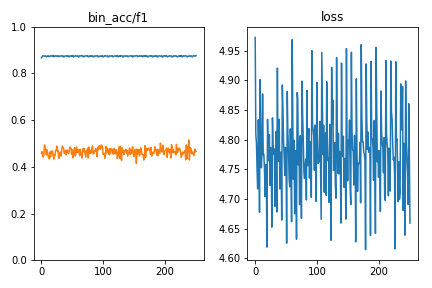
\includegraphics[width=0.6\textwidth]{images/final_model.png}
		\caption{Final Model (trained over 250 epochs)}
	\end{figure}
	\begin{itemize}
		\item 15 label F1: 0.467
		\item 14 label F1:  0.499
		\item Hamming loss: 0.123
	\end{itemize}
\end{frame}

\begin{frame}
	\frametitle{\overtitle}
	\framesubtitle{Sample Output}
	\begin{centering}
	\texttt{%
		0 0 0 0 0 0 0 0 0 1 0 0 0 0 \\
		0 0 0 0 0 0 0 0 0 1 0 0 0 0 \\
		0 0 0 0 0 0 0 0 0 1 0 0 0 0 \\
		0 0 0 0 0 0 0 0 0 1 0 0 0 0 \\
		0 0 0 0 0 0 0 0 0 1 0 0 0 0 \\
		0 0 0 0 0 0 0 0 0 1 0 0 0 0 \\
		0 0 0 0 0 0 0 0 0 1 0 0 0 0 \\
		0 0 0 0 0 0 0 0 0 1 0 0 0 0 \\
		0 0 0 0 0 0 0 0 0 1 0 0 0 0 \\
		0 0 0 0 0 0 0 0 0 1 0 0 0 0 \\
		...
		}
	\end{centering}
\end{frame}

\begin{frame}
	\frametitle{\overtitle}
	\framesubtitle{Confusion Matrix}
	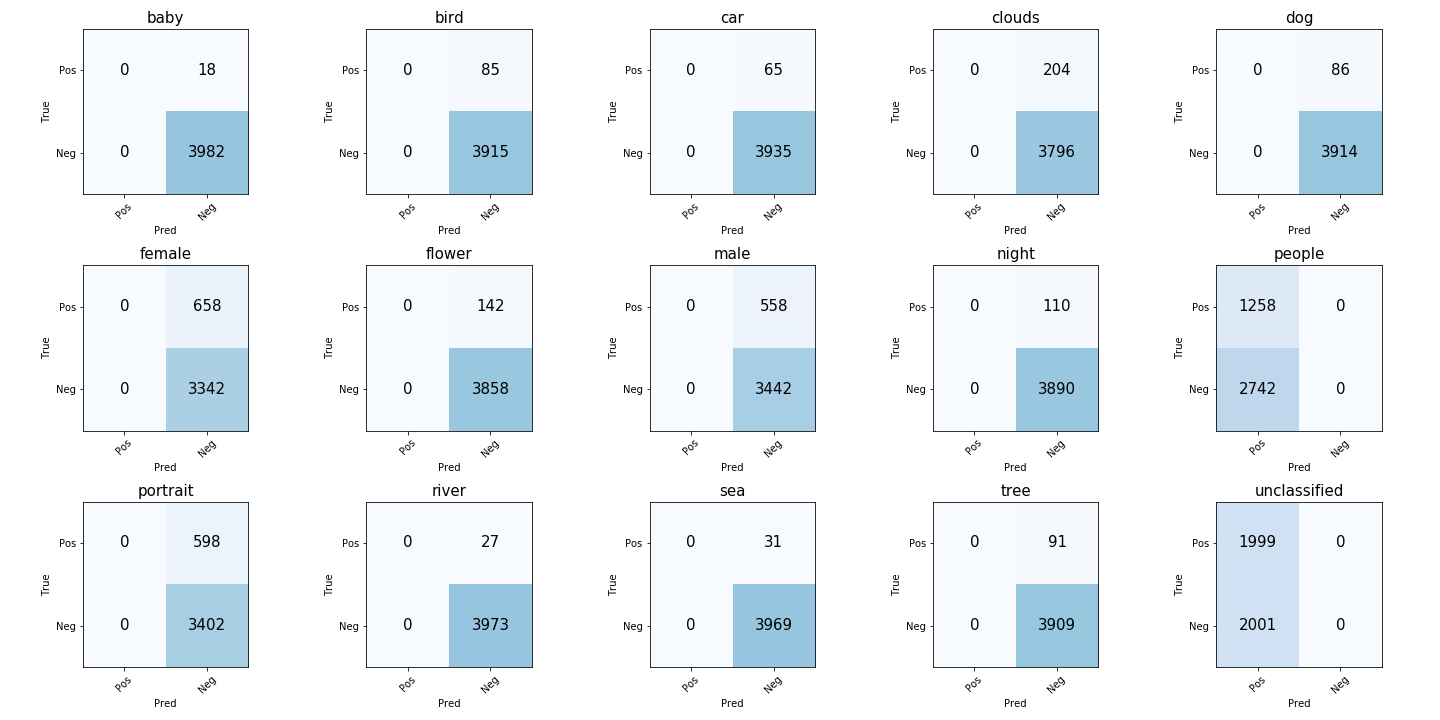
\includegraphics[width=\textwidth]{images/final_model_confusion.png}
	\begin{itemize}
		\item Always predicts same result for each label on every picture
	\end{itemize}
\end{frame}

